\documentclass[../main.tex]{subfiles}

\begin{document}

    \chapter{Growth and Solow Model}
        
        \section{Growth rates}
        We have by the chain rule that
        \begin{align}
            \frac{ d\ln{x(t)} }{ dt }
            = \frac{ 1 }{ x(t) } \frac{ dx(t) }{ dt }
            = \frac{ \dot{x}(t) }{ x(t) }
        \end{align}
        We call $\frac{\dot{x}(t) }{ x(t) }$ the growth rate of $x$. Suppose growth rate is constant at $g$, then
        
        \begin{align}
            \frac{d \ln(x(t))}{dt}
            = \frac{\dot x(t)}{x(t)} = g
            &\implies 
            d \ln(x(t)) = g \;dt
            \\
            &\implies 
            \int d \ln(x(t)) = \int g \; dt
            \\
            &\implies 
            \ln(x(t)) =  gt + c
            \\
            &\implies 
            x(t) =  e^{gt + c} = e^{gt}e^c = x(0)e^{gt}
            \\
            &\implies 
            x(t) = x(0)e^{gt}
        \end{align}
        
        \section{Solow Model}
        
        
        Firm production is a function of capital $K(t)$, and \textbf{effective labor} $A(t)L(t)$. $A(t)$ is technology and $L(t)$ is labor, which also represents \textbf{population}:
        \begin{align}
            Y(t) = F(K(t), A(t) L(t))
        \end{align}
        
        Assume production function is homogeneous of degree one:
        \begin{align}
            F(a K, a A L) = a F(K, A L)
        \end{align}
        
        Define capital and output \textbf{per effective labor} $k(t), y(t)$ as
        \begin{align}
            k(t) &= \frac{K}{AL},
            \\
            y(t) &= \frac{Y}{AL}
            = \frac{F(K, AL)}{AL}
            = F\left(\frac{K}{AL}, \frac{AL}{AL}\right)
            = F\left(\frac{K}{AL}, 1\right)
            = F(k, 1) = f(k),
        \end{align}
        which are also called \textbf{the intensive form} of capital and output, where $f'(k) > 0, \quad f''(k) < 0$.
        
    \section{Dynamics of model}
        
        Labor and technology have constant growth rates
        \begin{align}
            \frac{\dot A(t)}{A(t)} = g, \quad
            \frac{\dot L(t)}{L(t)} = n
        \end{align}
        
        Capital changes with \textbf{fixed exogenous rates} for savings $s$ and depreciation $\delta$:
        \begin{align}
            \dot K(t) &= sY(t) - \delta K(t).
        \end{align}
        
        Output that is not saved is consumed:
        \begin{align}
            C(t) &= (1-s)Y(t).
        \end{align}
        
        Then we have for effective capital
        \begin{align}
            k
            = \frac{K}{AL}
            &\implies
            \ln k = \ln K - (\ln A + \ln L)
            \\
            &\implies
            \underbrace{\frac{\dot k}{ k}}_{= d\ln(k) / dt}
            = \frac{\dot K}{K} - \left(\frac{\dot A}{A} + \frac{\dot L}{L}\right)
            \\
            &\implies
            \dot{k} =
            \underbrace{\frac{1}{AL}}_{=k/K} (sY - \delta K) - \left(g + n\right) k
            \\
            &\implies
            \dot k = s f(k) - (g + n + \delta) k
            \label{eqn:kdot-intensive}
            \\
            &\implies
            \dot y = \frac{d}{dt} f(k) = f'(k) \dot k,
            \quad f'(k) > 0.
            \label{eqn:ydot-intensive}
        \end{align}
        Equations \eqref{eqn:kdot-intensive} and \eqref{eqn:ydot-intensive} are the intensive form of law of motion for capital and income.
        
        
    \section{Balanced Growth Path}
        
        On the \textbf{balanced growth path (BGP)} we have that all growth rates are constant. Let $\frac{\dot k(t)}{k(t)} = g_k(t)$. Then on the BGP, constant $g_k(t)$ implies $\dot g_k(t) = 0$, which implies $\dot k(t) = 0$:
        \begin{align}
            \frac{\dot k}{k} = g_k(t)
            = s \frac{f(k)}{k} - (g+n+\delta)
            &\implies
            \overbrace{
                \frac{\dot g_k(t)}{g_k(t)}
            }^{
                \frac{d}{dt} \ln g_k(t)
            }
            = \frac{f'(k)\dot{k}}{f(k)} - \frac{\dot k}{k}
            = \left(\frac{f'(k)}{f(k)} - \frac{1}{k}\right)\dot{k}
            = 0
            \\
            &\implies
            \dot{k}
            = \frac{0}{(f'(k)/f(k) - 1/k)} = 0, \quad \frac{f'(k)}{f(k)} - \frac{1}{k} \ne 0.
        \end{align}
        
        \begin{figure}[!ht]
            \centering
            \begin{subfigure}
                \centering
                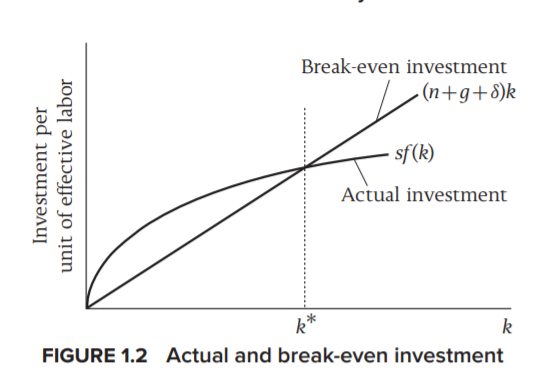
\includegraphics[width=0.4\linewidth]{subfile/attachments/1.1-actual_breakeven_investment.png}
            \end{subfigure}
            \begin{subfigure}
                \centering
                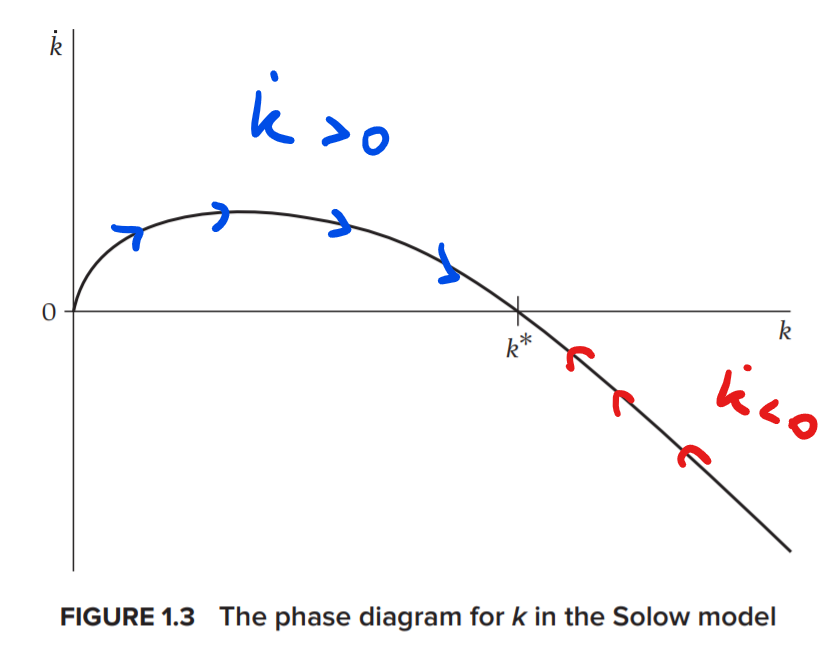
\includegraphics[width=0.4\linewidth]{subfile/attachments/1.2-phase diagram k.png}
            \end{subfigure}
        \end{figure}
        
        Then with the BGP level of capital $k^*$, we have
        \begin{align}
            \dot k(t) = 0
            &\implies
            sf(k^*) = sy^* = (g + n + \delta) k^*
            \\
            &\implies
            y^* = \frac{g+n+\delta}{s} k^*,
            \quad
            \dot y^* = \frac{g+n+\delta}{s} \dot k^* = 0,
    \end{align}
        
        and \textbf{income per capita} is equal to technology growth
        \begin{align}
            \tilde y = \frac{Y}{L} = y A
            &\implies
            \ln (\tilde y) = \ln y + \ln A
            \\
            &\implies
            \frac{\dot{\tilde y}}{\tilde y} = \frac{\dot y}{y} + \frac{\dot A}{A} = 0 + g = g.
        \end{align}
        
    \section{Golden-rule level of capital}
        
        Golden-rule level of savings and capital maximizes consumption on the BGP path. Assume Cobb-Douglas production,
        \begin{align}
            f(k) = k^\alpha.
        \end{align}
        
        Then on the BGP,
        \begin{align}
            f(k) = s k^{*\alpha} = (g + n + \delta) k^*
            \implies
            s = (g + n + \delta) k^{*1-\alpha}
        \end{align}
        
        BGP consumption given by
        \begin{align}
            c^*
            = (1-s)y^*
            &= [1 - (g + n + \delta) k^{*1-\alpha}] k^{*\alpha}
            \\
            &= k^{*\alpha} - (g + n + \delta) k^*
            .
        \end{align}
        
        Maximizing $c^*$ with respect to $k^*$, we have that
        \begin{align}
            \frac{\partial c^*}{\partial k^*}
            &= \alpha k_{GR}^{\alpha-1}
            - (g + n + \delta)
            = 0
            \\
            \implies
            k_{GR}
            &= \left(\frac{g + n + \delta}{\alpha}\right)^{\frac{1}{\alpha-1}}
            \\
            \implies
            s_{GR} &= \alpha.
        \end{align}

\end{document}